\documentclass[conference]{IEEEtran}
\usepackage{graphicx}
\usepackage{amsmath}
\usepackage{url}
\title{Dry Bean Classification for Sustainable Sorting Using Introductory Machine Learning}
\author{\IEEEauthorblockN{Abdulrahman Alfawaz}\IEEEauthorblockA{Prince Sultan University\\CS316: Introduction to AI and Data Science, Term 261}}
\begin{document}
\maketitle
\begin{abstract}
This project investigates whether simple supervised learning methods can classify dry bean varieties using geometric measurements. The UCI Dry Bean dataset contains 13,611 records with 16 predictors and seven target classes. After removing 68 exact duplicates, an 80/20 stratified split reserves 2,709 observations for final testing. Logistic regression, K-nearest neighbors and a decision tree are compared using five-fold cross-validation on the training set. Standardization is fitted within each validation fold. Logistic regression obtains the highest mean macro F1, although its advantage over K-nearest neighbors is very small. The selected model achieves 92.14\% test accuracy and 0.9316 macro F1, compared with a 26.17\% majority-class baseline. An illustrative confidence rule refers 14.65\% of records for human review. The project connects classification to efficient agricultural sorting and responsible production, while distinguishing measured predictive performance from potential environmental benefits.\end{abstract}
\begin{IEEEkeywords}classification, sustainable agriculture, logistic regression, data preprocessing, dry beans\end{IEEEkeywords}
\section{Introduction}
Agricultural sorting involves identifying products consistently so that downstream handling can follow their intended variety. This project studies a bounded version of that problem: predicting one of seven dry bean varieties from numerical measurements. It applies the CS316 workflow of loading a dataset, exploring its structure, preparing features, fitting models and evaluating predictions on unseen examples.

The UCI dataset provides measurements extracted from bean images by the original researchers \cite{uci}. Therefore, this project begins with a tabular dataset. Building a camera, extracting image features and controlling physical sorting machinery are outside the implemented scope. This scope makes the work feasible for an individual student while retaining an end-to-end data science experiment.

The sustainability motivation relates to responsible production and resource use. SDG 12 includes efficient management of natural resources and reductions in food losses along supply chains \cite{sdg}. More consistent identification could support appropriate handling and reduce avoidable sorting errors. However, the present data contain neither waste quantities nor operational energy measurements. Consequently, the environmental contribution is a proposed application that requires field measurement.

The research questions are whether introductory classifiers can exceed a majority baseline, whether class-level evaluation reveals uneven performance, and how a simple human-review rule changes the balance between automation coverage and prediction reliability. All experimental choices are recorded in executable code.
\section{Dataset and Exploratory Analysis}
\subsection{Data source and variables}
The dataset is attributed to Koklu and Ozkan and is distributed through UCI under CC BY 4.0 \cite{uci}. The supplied CSV preserves the original table. It has 16 numerical predictors and a categorical target named Class. Examples of predictors include area, perimeter, major and minor axis length, compactness and shape factors. The feature names in the source files are preserved for reproducibility.

Area represents the number of pixels within the bean region. Axis lengths describe its dimensions. Compactness summarizes a relationship between equivalent diameter and major axis length. These measurements provide a natural connection to the course's discussion of numerical features and similarity. The dataset has no personal identifiers, although this alone does not establish suitability for every agricultural setting.

The seven classes are BARBUNYA, BOMBAY, CALI, DERMASON, HOROZ, SEKER and SIRA. Table~\ref{tab:counts} shows the cleaned distribution. The largest class is approximately 6.8 times the smallest. This imbalance motivates macro F1 in model selection because a high aggregate accuracy can hide weaker performance on a less common variety.
\begin{table}[ht]\caption{Class distribution after exact deduplication}\label{tab:counts}\centering
\begin{tabular}{lr}\hline Class & Records\\\hline
BARBUNYA &1322\\ BOMBAY &522\\ CALI &1630\\ DERMASON &3546\\ HOROZ &1860\\ SEKER &2027\\ SIRA &2636\\\hline Total &13543\\\hline\end{tabular}\end{table}
\subsection{Quality checks}
Pandas checks confirm zero missing values and 68 exact duplicate rows. Removing duplicate rows before partitioning reduces the risk of identical records appearing in training and testing. Identical measurements can sometimes describe distinct physical objects, so deduplication is a conservative experimental choice rather than proof of faulty collection. The original data remain included for inspection.

No imputation is performed because there are no missing values. The code deliberately raises an error if missing values appear in a changed dataset, prompting inspection instead of silently producing different results. Outliers are retained because size extremes may describe genuine varieties. Deleting these observations without domain evidence could distort the target distribution.

Figure~\ref{fig:distribution} uses training data to show representation across classes. Figure~\ref{fig:scatter} plots two training features and shows both separation and overlap. These plots support exploratory interpretation, while final generalization claims come from the reserved test set.
\begin{figure}[ht]\centering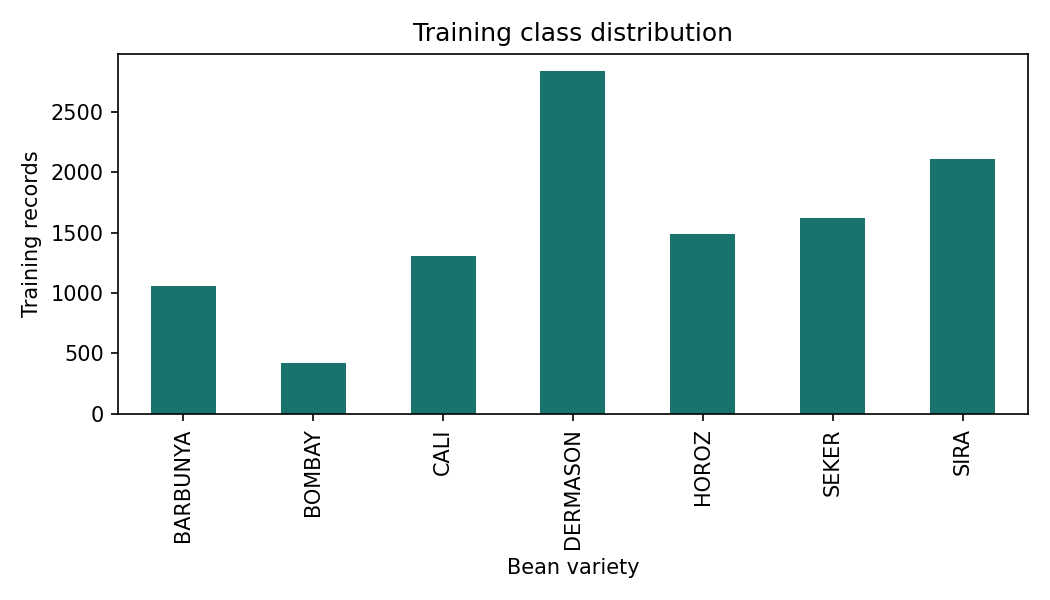
\includegraphics[width=\columnwidth]{results/class_distribution.png}\caption{Training class counts after stratified splitting. Representation remains uneven, motivating macro-averaged evaluation.}\label{fig:distribution}\end{figure}
\section{Methodology}
\subsection{Partitioning and preprocessing}
The cleaned data are split into 10,834 training records and 2,709 test records using a random seed of 42. Stratification approximately preserves class proportions. The seed supports repeatability. This is a random record-level split, so the experiment assesses generalization to records from the same source distribution. It does not establish transfer to a new farm or imaging system.

For each numerical feature, standardization computes
\begin{equation}z_j=(x_j-\mu_j)/\sigma_j.\end{equation}
The mean and standard deviation are learned from the training portion of each cross-validation fold. A scikit-learn pipeline combines the scaler and classifier, so validation observations never determine the preprocessing parameters. After model selection, the pipeline is fitted on the complete training set and reused for test predictions. This implements the leakage prevention principles in the course normalization slides \cite{course}.

Scaling is especially relevant to KNN because distances otherwise depend heavily on feature units. It also helps numerical optimization in logistic regression. A decision tree ordinarily does not need standardization, but the same pipeline structure is used for a consistent experiment. The transformation preserves the ordering on which tree splits depend.
\subsection{Candidate models}
Logistic regression models class probabilities from a weighted combination of the standardized features. Its inverse regularization parameter C is searched over 0.1, 1 and 10. The iteration limit is 3,000. Larger C allows weaker regularization within this specific search.

KNN predicts using neighboring training records. Values of k equal to 3, 5 and 9 are compared, with uniform voting and the default Euclidean distance. This connects directly to similarity measures. A decision tree forms feature-based rules, and maximum depths of 5, 10 and unrestricted are compared. Its random seed is fixed at 42.

Each candidate configuration receives the same five stratified folds. The score is macro F1. Nine configurations and five folds require 45 validation fits, followed by refitting each family's best configuration. This small search is practical for a laptop and keeps the experiment understandable. The scikit-learn implementation supports the pipelines and model selection \cite{sklearn}.
\subsection{Evaluation design}
The winning family is chosen by mean validation macro F1 using training data only. The test set is evaluated after that selection. A DummyClassifier that always predicts the most frequent training label provides a baseline on the identical test set.

Accuracy is the fraction of correctly predicted test records. Precision measures the reliability of predictions for a class, while recall measures the proportion of that class that is recovered. For each class,
\begin{equation}F_1=2\frac{\mathrm{precision}\,\mathrm{recall}}{\mathrm{precision}+\mathrm{recall}}.\end{equation}
Macro F1 is the unweighted mean across the seven classes. It gives the small BOMBAY class the same importance as DERMASON. The confusion matrix records actual classes in rows and predicted classes in columns.

An approximate 95\% interval for accuracy is obtained from 1,000 bootstrap resamples of the fixed test predictions using seed 42. This estimates sampling uncertainty conditional on the trained model. It does not include all uncertainty from training, alternative splits or external deployment.
\begin{figure}[ht]\centering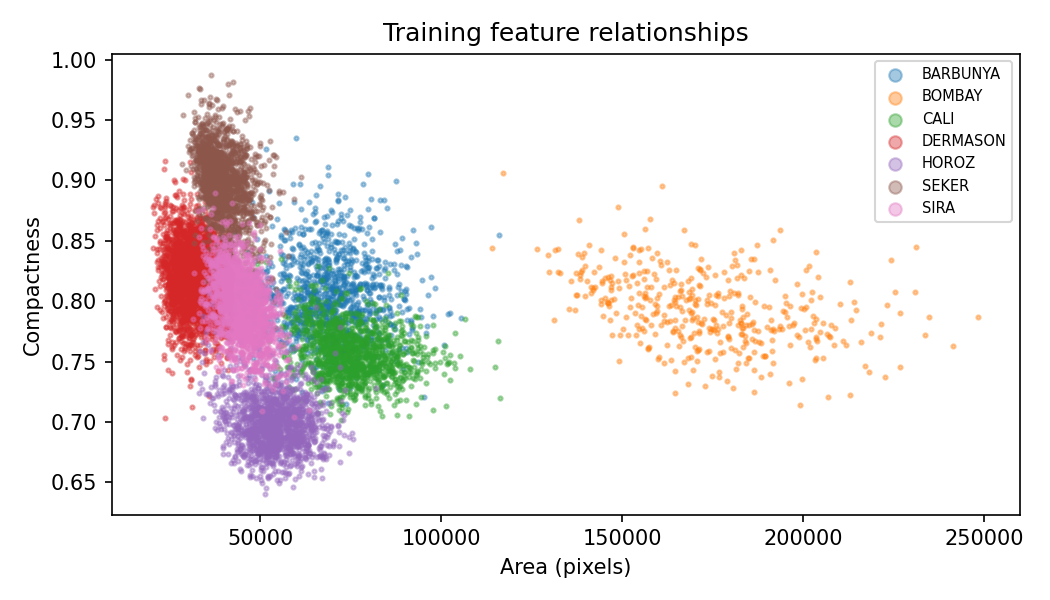
\includegraphics[width=\columnwidth]{results/feature_scatter.png}\caption{Area and compactness in the training set. Some varieties overlap in this two-feature view, supporting use of the full feature set.}\label{fig:scatter}\end{figure}
\section{Results and Main Insights}
\subsection{Training-only model selection}
Table~\ref{tab:models} reports the selected configuration within each family. Logistic regression with C=10 obtains mean macro F1 of 0.9368. KNN with nine neighbors obtains 0.9367 and a depth-10 tree obtains 0.9209. The difference between logistic regression and KNN is only about 0.00009, much smaller than their fold-to-fold standard deviations. The selection rule chooses logistic regression, but these results do not establish meaningful statistical superiority over KNN.
\begin{table}[ht]\caption{Five-fold training validation results}\label{tab:models}\centering\begin{tabular}{lrr}\hline Model & Macro F1 & Std. dev.\\\hline Logistic, C=10 &0.9368&0.0035\\KNN, k=9&0.9367&0.0046\\Tree, depth=10&0.9209&0.0019\\\hline\end{tabular}\end{table}
\subsection{Reserved test performance}
The selected model achieves 92.14\% accuracy and macro F1 of 0.9316. The majority baseline obtains 26.17\%. The absolute improvement over that baseline is 65.97 percentage points. The approximate bootstrap interval is 91.10\% to 93.21\%. These numbers are generated directly by the supplied script, and individual predictions are exported to CSV.

Table~\ref{tab:classes} shows the class-specific test results. BOMBAY has the strongest F1 at 0.9952, with support of only 104 test records. SIRA has the weakest F1 at 0.8756, including precision of 0.8635. The variation shows why a single accuracy value is insufficient to describe the model. Higher performance for a small class can occur when its geometry is distinctive, while overlapping measurements can make a common class harder.
\begin{table}[ht]\caption{Test results for the selected model}\label{tab:classes}\centering\begin{tabular}{lrrr}\hline Class &Precision&Recall&F1\\\hline BARBUNYA&0.9294&0.8943&0.9115\\BOMBAY&1.0000&0.9904&0.9952\\CALI&0.9056&0.9417&0.9233\\DERMASON&0.9255&0.9111&0.9183\\HOROZ&0.9695&0.9409&0.9550\\SEKER&0.9367&0.9483&0.9425\\SIRA&0.8635&0.8880&0.8756\\\hline\end{tabular}\end{table}

Figure~\ref{fig:confusion} makes errors visible across varieties. The diagonal contains correct predictions. Off-diagonal cells indicate which varieties would require additional review or measurement. Error analysis should guide future data collection, particularly examples near the overlapping class boundaries.
\begin{figure}[ht]\centering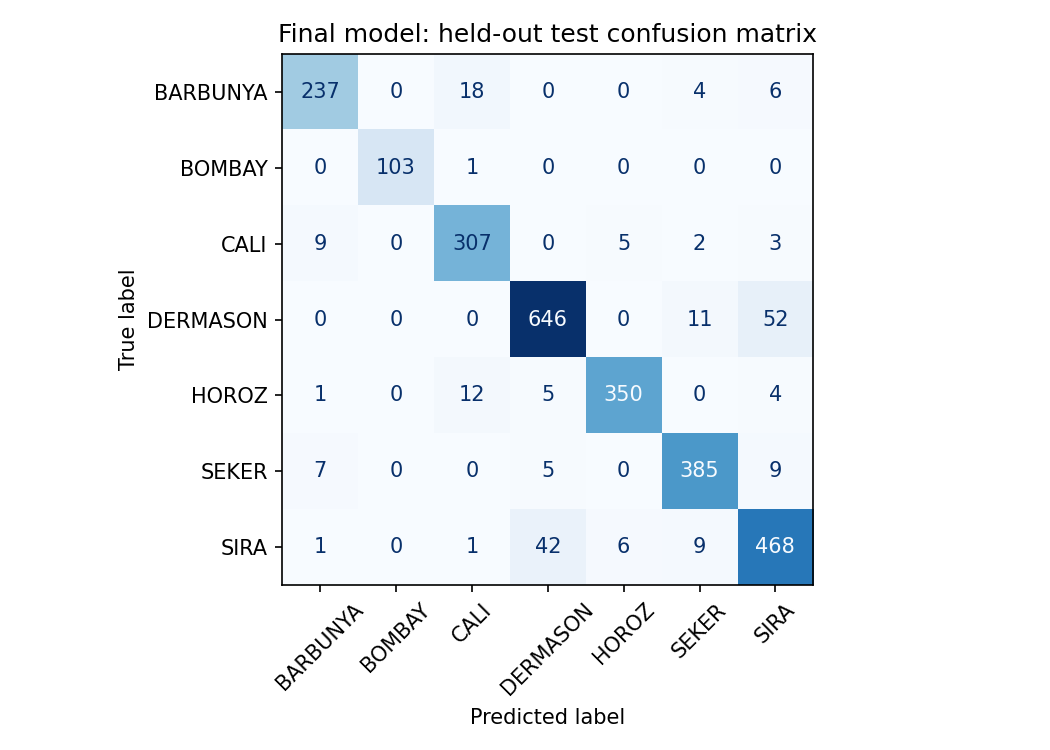
\includegraphics[width=\columnwidth]{results/confusion_matrix.png}\caption{Held-out test confusion matrix for logistic regression. Rows show actual varieties and columns show predictions.}\label{fig:confusion}\end{figure}
\subsection{Simple customization for human review}
A fixed rule accepts a prediction only when the largest predicted class probability is at least 0.80. It refers all other records for human review. The threshold is specified in the code and is not optimized against test outcomes. It accepts 85.35\% of test records, with accuracy of 97.10\% among accepted records, and refers 397 cases.

This result describes a coverage-reliability tradeoff. It does not change overall test accuracy to 97.10\%, because the deferred records still require a decision. The cost and quality of that human decision are unmeasured. Predicted probabilities have also not undergone a calibration study, so 0.80 should be treated as an illustrative rule. A deployed threshold would require validation against operating costs and review capacity.
\section{Ethical Considerations and Sustainability}
The dataset supports classification of known varieties. Using a predicted label as a direct reason to discard food would require a separate justification and safeguards. Incorrect labels could affect growers, buyers and processing decisions. Human review for uncertain records provides a simple design response, although this experiment does not measure its operational effectiveness.

The public data contain no human subjects or personal identifiers. Remaining concerns include representation of local varieties, changes in imaging conditions and unequal errors across classes. A model trained on these seven classes will still assign a label to an unfamiliar variety. It therefore requires additional controls and external testing before physical deployment.

The sustainability connection is a hypothesis about better handling and sorting consistency. Potential gains should be assessed using actual rejected mass, rework rates, energy consumption and operator time. Classification accuracy alone cannot establish lower carbon emissions, reduced water use or less food waste. A useful follow-up would compare these outcomes with a manual sorting baseline in a controlled pilot.
\section{Conclusion and Future Work}
A compact supervised learning workflow achieves 92.14\% held-out accuracy on the cleaned Dry Bean dataset. Logistic regression and KNN perform almost identically in cross-validation, while logistic regression wins under the predetermined selection rule. Class-specific metrics reveal that some varieties remain more difficult than others.

The project applies Pandas, exploratory plots, preprocessing, normalization, classification and evaluation from CS316. It adds a small validation search and human-review analysis without requiring a complex application. Future work should collect data from new settings, examine probability calibration, compare alternative review thresholds using validation data, and measure resource outcomes in an actual sorting process.
\appendices
\section{Memory Optimization and Reproduction}
The dataframe occupies 2,584,030 bytes after deduplication and before optimization. Converting numerical predictors to float32 and the repeated Class strings to categorical storage reduces measured dataframe memory to 989,322 bytes, a reduction of 61.71\%. The measurement includes the index and deep object accounting through Pandas. It describes dataframe storage, not peak process memory or the internal allocations of model fitting.

The relevant code is reproduced below. It appears in project.py before splitting. A fixed dtype conversion requires no learned statistics from the test set. Float32 reduces numerical precision, and the supplied reported results are obtained using that conversion throughout.
{\footnotesize
\begin{verbatim}
before = int(df.memory_usage(deep=True).sum())
df[features] = df[features].astype("float32")
df["Class"] = df["Class"].astype("category")
after = int(df.memory_usage(deep=True).sum())
\end{verbatim}
}
The implementation also reuses a single dataframe, performs column-wise operations, uses a limited grid and runs fits with n\_jobs=1 to limit simultaneous copies. The script saves summary.json, validation metrics, a classification report, individual test predictions and four plots. The dependency versions are pinned in requirements.txt. Running python project.py regenerates these outputs from the bundled CSV.
\section{AI Use and Originality Statement}
ChatGPT assisted with selecting the topic, writing and executing the analysis code, interpreting the outputs, drafting the report and preparing presentation material. The author must review the deliverables, verify understanding and comply with the instructor's rules before submission. The numerical results were produced by executing the included code. No institutional plagiarism check or AI-detection score has been obtained, and no percentage is asserted. Dataset and conceptual sources are attributed below.
\begin{thebibliography}{4}
\bibitem{uci} M. Koklu and I. A. Ozkan, ``Dry Bean,'' UCI Machine Learning Repository, 2020, doi: 10.24432/C50S4B. [Online]. Available: \url{https://archive.ics.uci.edu/dataset/602/dry+bean+dataset}. Accessed: Nov. 16, 2026.
\bibitem{sdg} United Nations, ``Goal 12: Responsible consumption and production.'' [Online]. Available: \url{https://sdgs.un.org/goals/goal12}. Accessed: Nov. 16, 2026.
\bibitem{course} CS316, ``Introduction to AI and Data Science,'' course slides supplied by the student, Prince Sultan University, Term 261. Topics include Pandas, missing data, normalization, classification and similarity measures.
\bibitem{sklearn} F. Pedregosa et al., ``Scikit-learn: Machine learning in Python,'' Journal of Machine Learning Research, vol. 12, pp. 2825--2830, 2011.
\end{thebibliography}
\end{document}
